\chapter{Implementacion}
\label{chapter:implementation}

El siguiente conjunto de secciones describen la implementacion del metodo
propuesto segun las explicaciones presentadas en el Capitulo
\ref{chapter:proposed-method}. La implementacion propuesta utiliza un software
de simulacion como el mostrado en \cite{} (\url{}), este software de simulacion esta
programado en Unity con codigo fuente en lenguaje C\# de Visual Studio.

\section{Codificando los diccionarios de piezas}
\label{section:piece_dictionary}

La primera parte que se desarrollo para poder integrar el listado de piezas al
sistema de generacion fue decir la manera en como se establecerian las
diferentes piezas como las mostradas en la figura \ref{figure:game-basic-blocks}
del Capitulo \ref{chapter:proposed-method}, para esto se tomaron enncuenta
varias posibilidades, la primera, como se explica en la seccion
\ref{subsection:objectorientedidea} se buscaba ordenar las diferentes piezas
como diccionarios que contuvieran una o mas referencias a las piezas que
integraban cada entrada del diccionario, para esto las primeras 11 posiciones
eran elementos individuales uno para cada pieza como el mostrado en la figura
\ref{code:dic_individual_piece}, en el codigo se aprecia la manera en como se
designaba una pieza del juego, para poder trabajar de manera dinamica para poder
agregar mas compuestos segun fuese necesario se utilizaban dos diccionarios
extra, estos contenian los datos de los tipos de materiales posibles y la
informacion de los tamaños de las piezas, de esta manera en caso de tener mas de
una pieza en algun punto del diccionario era posible modificar el valor de
offset de cada una de las piezas calculando la distancia del punto central de
cada pieza al centro de todo el conjunto.

\begin{listing}[t]
  \begin{minted}[frame=lines, framesep=2mm,baselinestretch=1.2,fontsize=\footnotesize,linenos]{python}
    BLOCKS = {
      0: [
          {'type': BLOCK_TYPE['Circle'],
          'material': BLOCK_MATERIAL['wood'],
          'offset': [0, 0, 0] # x, y, z - Calculated from the center of the figure
          }]
    }

    BLOCK_TYPE = {
    'Circle': {'height': 72, 'lenght': 72},
    'RectTiny': {'height': 22, 'lenght': 42},
    'RectSmall': {'height': 22, 'lenght': 42},
    'RectBig': {'height': 22, 'lenght': 42},
    'RectMedium': {'height': 22, 'lenght': 42},
    'RectFat': {'height': 42, 'lenght': 82},
    'SquareTiny': {'height': 22, 'lenght': 22},
    'SquareSmall': {'height': 42, 'lenght': 42},
    'Triangle': {'height': 72, 'lenght': 72},
    'TriangleHole': {'height': 82, 'lenght': 82},
    'SquareHole': {'height': 82, 'lenght': 82}
    }

    BLOCK_MATERIAL = {
        'wood': 0,
        'stone': 1,
        'ice': 2
    }
  \end{minted}
  \caption{Ejemplo de diccionario con un solo elemento}
  \label{code:dic_individual_piece}
\end{listing}

De esta manera como se explico anteriormente era mas sencillo crear compuestos,
sin embargo, la desventaja que conyevaba utilizar este metodo era que no podiar
realizar modificaciones a las restricciones de las piezas, es decir, en caso de
querer evitar que un conjunto de piezas con determinados materiales no fuesen
generados no se tenia la facilidad de impedir este tipo de combinaciones.

En luz de esta informacion se opto por utilizar el metodo en base a clases
mencionado en la seccion \ref{subsection:classorientedidea}, el codigo
\ref{code:dic_individual_piece} muestra la nueva estructura utilizada segun el
diagrama de clases presentado en la figura \ref{figure:pieces-class-diagram},
deacuerdo a el diagrama presentado una clase base con las operaciones y
propiedades necesarias funcionaria como una clase \textit{padre} para las clases
de piezas particulares, de esta manera los individuos se representaran como un
conjunto de referencias a las clases que deben de ser generadas para la
composicion de niveles, sin embargo, esta manera de representar a los individuos
no contempla las restricciones que pueden ser definidas para la combinacion de
piezas-materiales, debido a esto se opto por genar una lista global que
mantuviera un record de las restricciones aplicadas en el sistema, y al momento
de generar cada reinstanciacion de clase para los indiciduos esta informacion se
pasara a las clases segun fuese requerido, en el codigo se presenta una variable
con el nombre \textit{mat}, esta variable tomara una lista de 3 valores que
define si alguno o algunos de los materiales no puede ser utilizado al momento
de asignar las clases a los individuos, al momento de encontrar una pieza que de
la coincidencia no puede ser utilizada con ningun material se eliminaran los
datos de la pieza generada y se pedira al sistema genere otra de manera aleatoria.

\begin{listing}[ht]
  \begin{minted}[frame=lines,framesep=2mm,baselinestretch=1.2,fontsize=\footnotesize,linenos]{python}
    class Circle(Piece):
      def __init__(self, mat, x=0, y=0, r=0):
          self.Name = "Circle"
          self.Height = 75
          self.Width = 75
          Piece.__init__(self, x, y, r, mat)
          self.update_values()
  \end{minted}
  \caption{Ejemplo de estructura de las clases hija que heredan de la principal}
  \label{code:dic_individual_piece}
\end{listing}


\section{Creacion de compuestos}
\label{section:composite_creation}

Una vez definidas las clases particulares que controlaran la informacion de las
piezas en el algoritmo se procede a definir la manera en como se entregaran y
controlaran los diferentes compuestos de piezas, para terminos mas simples los
compuestos son grupos de una o mas piezas y se mostraran a manera de diccionario
de listas como se muestra en el codigo \ref{code:dic_composites}, de esta manera
cada entrada en el diccionario tiene por nombre o apuntador el valor posicion
segun se fueron agregando al diccionario mientras que el contenido es una lista
con tuplas donde se estipula la informacion pertinente de cada pieza en el
compuesto, un ejemplo claro es el elemento en la posicion \textit{9} el cual
cuenta con 3 piezas que muestran los valores de offset medida desde el centro
del compuesto visto graficamente en el juego, esta lista se utiliza para
mantener un control de los compuestos que se pueden ir agregando durante la
ejecucion del algoritmo, de tal manera que las clases auxiliares de
\textit{Composite} creadas haran referencia a una o mas piezas segun la lista se
haya proporcionado al crear el compuesto.

\begin{listing}[ht]
  \begin{minted}[frame=lines,framesep=2mm,baselinestretch=1.2,fontsize=\footnotesize,linenos]{python}
    Composites = {
      0: [("RectTiny", 0, 0, 0, "wood")],
      1: [("RectSmall", 0, 0, 0, "wood")],
      2: [("RectMedium", 0, 0, 0, "wood")],
      3: [("RectBig", 0, 0, 0, "wood")],
      4: [("RectFat", 0, 0, 0, "wood")],
      5: [("SquareSmall", 0, 0, 0, "wood")],
      6: [("SquareHole", 0, 0, 0, "wood")],
      7: [("Circle", 0, 0, 0, "wood")],
      8: [("TriangleHole", 0, 0, 0, "wood")],
      9: [("RectBig", 100, 5, -27, "wood"), ("RectBig", -100, 5, 27, "wood"), ...
            ...("RectSmall", 0, 0, 90, "wood")]
    } 
  \end{minted}
  \caption{Diccionario con los compuestos existentes}
  \label{code:dic_composites}
\end{listing}

\section{Definicion de clase auxiliar de individuo}
\label{section:definition_of_clases}

Mediante el uso de la clase de composite se tiene un mejor control de los genes
que conformaran cada individuo de la poblacion, una vez que se tiene este
aspecto controlado el siguiente paso es el de crear programar la clase que
llevara el control de los cromosomas de un individuo, siendo los cromosomas los
compuestos asignados a cada individuo particular, de tal manera que un individuo
dentro de la informacion de cromosomas hara referencia a otra lista de
compuestos, la manera en como un \textit{Individuo} relaciona los compuestos es
mediante el uso de la linea de codigo:

\begin{minted}{python}
  chromosome_objects = [Composite(Composites[composite]) for composite in self.chromosome]
\end{minted}

Mediante esta linea de codigo se indica que se debera de crar una lista en donde
cada elemento sera una instancia de un compuesto asignado al individuo, de esta
manera si se requiere modificar la posicion o materiales de un compuesto
particular en el individuo es posible hacerlo desde la clase de
\textit{individuo}, de igual manera esta clase tiene como funciones principales
como se muestran en el diagrama de clase de la figura
\ref{figure:individual-class-diagram} realizar los calculos de fitness y generar
las listas de piezas que seran utilizadas para generar los archivos de salida
necesarios para las simulaciones de los niveles generados.



\section{Generacion de individuos}
\label{section:ind_generation}

Una vez definida la manera de controlar las clases el paso siguiente es el de
comenzar con la generacion de ls individuos de la poblacion, para poder lograr
esto se creo una linea de codigo en la cual los puntos necesarios para la
generacion de los individuos se entregan totalmente, esta linea de codigo en
cuestion es como sigue: 

\begin{minted}{python}
  pop = [Individual(chromosome = get_random_chrom(ind_pieces), ..
    ..mask = create_new_mask(ind_pieces)) for i in range(population)]
\end{minted}

Mediante el uso de esta linea de codigo se le indica al sistema que se requiere
una lista que representara a los individuos de la poblacion, cada elemento de
esta lista sera una instancia independiente de la clase \textit{Individual},
para generar esta instancia de clase es requerido dos valores siendo estos
primero una lista de valores numericos que representan cuales piezas se
asignaran a los individuos, para generar esta lista se utiliza una funcion como
se muestra en el codigo \ref{code:get_random_chrom}, el segundo dato requerido
es una segunda lista que denota una mascara mediante la cual las piezas
asignadas seran acomodadas al momento de generar los archivos de simulacion,
finalmente la ultima seccion del codigo - \textit{for i in range(population)} -
denota que el proceso se debera de repetir una cierta cantidad de veces, es
decir que pada cada individuo se generara una instancia con valores diferentes a
los anteriores, la cantidad de vences que se debera de repetir depende de la
cantidad de individuos con los que se quiere estar trabajando en el algoritmo en
el caso de las pruebas realizadas se utilizo un totoal de 10 individuos lo que
significa que la lista \textit{pop} generada consta de 10 instancias diferentes
de la clase \textit{Individual}. 

Para la generacion de la lista de piezas o cromosomas asignados a un individuo
mostrada en la parte (1) del codigo en \ref{code:get_random_chrom}, aqui el
valor que se recive denota la cantidad de piezas o compuestos que se deberan de
asignar en la lista para el individuo, para asignar estos valores primero se
obtine un numero aleatorio que va desde \textit{0} hasta la cantidad de piezas o
compuestos presentes en la lista menos una unidad para evitar errores de
posicionamiento de lista, posteriormente se revisa si la pieza seleccionada
puede ser utilizada almenos en una combinacion dentro de la generacion, en caso
de que no puede ser utilizada se obtiene otra y de igual manera se revisa, en
caso de poder ser utilizada se agrega a la lista y avanza un contador para saber
cuando se llegue al limite de piezas posibles de usar, finalmente se entrega la
lista de piezas para la generacion de la instancia de clase. Para la generacion
de la mascara de acomodo de piezas se utiliza la seccion de codigo mostrado en
la parte (2), en esta parte lo que se realiza es que se revisa la cantidad de
compuestos que se pueden utilizar como en la parte anterior, este valor se
utiliza posteriormente para generar una lista aleatoria, la lista que se genera
tiene un total de 7 posiciones que denotan 7 divisiones que se realizan en el
area de un nivel para el acomodo de las piezas, mediante el uso del valor de
piezas en cada individuo se realiza una aleatorizacion de numeros desde
\textit{0} hasta la cantidad maxima de piezas, una vez se obtienen estos valores
aleatorios se revisa si la suma de estos da la cantidad de piezas en el
individuo, en caso de que no sea asi se repite el proceso, en caso de que si se
cumpla entonces la lista se regresa para la creacion de la instancia de clase.

\begin{listing}[ht]
  \begin{minted}[frame=lines, framesep=2mm, baselinestretch=1.2, fontsize=\footnotesize, linenos]{python}
 (1)  def get_random_chrom(sl):
        asl = 0
        chrom = []
        while asl < sl:
            prop = random.randint(0, len(Composites)-1)
            if clases[Composites[prop][0][0]].Valid == True:
                chrom.append(prop)
                asl += 1
        #random.randint(0,len(Composites)-1) for p in range(ind_pieces)
        return chrom

 (2)  def create_new_mask(pieces):
        div_list =[]
        while True:
            div_list = [random.randint(0, pieces-1) for col in range(7)]
            if sum(div_list) == pieces:
                break
          
        return div_list
  \end{minted}
  \caption{Codigo de asignacion de cromosomas(piezas)[1] y codigo para generar mascaras [2]}
  \label{code:get_random_chrom}
\end{listing}

Una vez que se ah logrado cear la lista de individuos se procede a inicializar
el algoritmo evolutivo, este algoritmo se ejecutara una determinada cantidad de
veces que se haya establecido en el codigo, el pseudo-codigo ah ejecutar con su
respectiva implementacion en codigo se enlista a continuacion en el codigo
\ref{code:algorithm_pseudocode}, este pseudocodigo engloba los aspectos
principales del sistema de generacion de niveles, el codigo se explica mas a
detalle en las secciones siguientes.

\begin{listing}[ht]
  \scalebox{.8}{\noindent%
\begin{Heardlisting}{%
   \begin{tabular}{r}% 
      Integrar miembros "elite" (1-4)\\ \\  \\  \\  \\
      Simular individuos (6)\\  \\
      Calcular fitness (8-9)\\  \\  \\
      Obtener padres de la generacion (10)\\  \\
      Realizar crossover (12)\\ \\
      Seleccionar elite (14-15)\\ \\
   \end{tabular}
}
if elite not null
   for member in elite
      population <- member
      trim population

execute process (game)

for individual in population
   individual.getfitness

parents <- selector_operator(population, required)

crossover_operation(population, parents)

population.order('fitness')
elite.add(population[1])
\end{Heardlisting}}
  \caption{Pseudo-codigo del algoritmo genetico}
  \label{code:algorithm_pseudocode}
\end{listing}

\subsection{Integracion de miembros elite}
\label{subsection:elite_member_integration}

Esta parte se encarga de iniciar los bucles de generacion, la funcion principal
de este broque de codigo es la revisar la lista auxiliar de miembros de elite
que existe en memoria, en caso de tener elementos en la lista estos se integran
a la lista de la poblacion integrandose al inicio de la misma, una vez agregados
todos los miembros la lista de la poblacion se corta hasta el numero maximo de
miembros permitidos en las generaciones, este valor se asigna como un valor de
entrada al inicio del archivo que contiene el codigo.

Una vez terminada esta accion se procede a denotar la cantidad de padres que
seran necesarios para generar los hijos de las generaciones futuras, esto se
hace mediante el calculo:
\begin{minted}{python}
  many = len(pop) * per_cross
\end{minted}
En donde \textit{pop} representa la lista de miembros de la poblacion,
\textit{per\_cross} representa un valor entre \textit{0\.0} y \textit{1\.0}, este
valor representa que tanto porcentaje de la poblacion se quiere realice cruces,
de esta manera la variable \textit{many} representa la cantidad de individuos
que se deberan de utilizar para cumplir el porcentaje de cruce, debido a que el
valor de \textit{per\_cross} puede generar un valor flotante se tiene una parte
de codigo en donde si el total de individuos que realizaran cruces es un numero
inpar entonces el valor que se debera de utilizar sera el numero par redondeado
hacia abajo, es decir, si de 10 individuos en la poblacion se quiere que un
total de individuos cercano al \textit{50\%} realizen un cruce entonces el valor
resultante para la variable \textit{many} seria de 5, en este caso lo que se
hace es restar 1 al resultado y despues se redondea hacia abajo, lo cual haria
que el numero de padres requeridos para los cruces sea de 4.

Una vez que se tiene el valor de los padres requeridos para los crces de la
generacion se procede a crear los archivos auxiliares de los individuos de la
poblacion, los archivos generados son en formato \textit{XML}, la informacion
que contienen estos archivos es la posicion, tipo y material de ls piezas que
seran utilizadas en el nivel, ademas de esto tambien contiene la informacion de
la cantidad y tipo de aves asi como de los enemigos que seran colocados, estos
archivos son almacenados en un folder en donde el software de simulacion se
encarga de obtenerlos y entregar los resultados despues de la simulacion.

Una vez que los archivos de simulacion han sido generados el algoritmo manda un
comando que manda la ejecucion del software de simulacion, el software en
particular cuenta con una ventan grafica en la que se puede apreciar los niveles
que se generaron o envolucionaron an caso de estar simulando archivos de una
generacion despues de la primera, de igual manera el software genera un archivo
en formato \textit{XML} similar al que se genera antes de la simulacion, la
diferencia entre ambos archivos es que el que es entregado despues de la
simulacion entrega los datos de posicion del ultimo estado registrado del nivel,
ademas de que se puede solicitar que entregue el valor de la aceleracion de la
misma, el valor de aceleracion es tomado en cuenta desde el punto en el que la
pieza comienza su descenso, en caso de que una pieza sea destruida durante el
proceso de simulacion ninguno de los datos de esa pieza son grabados en los
archivos, la manera de llevar control de las piezas que entran y las que salen
es mediante el uso de un numero de lista asignado al momento de generar los
archivos de simulacion de la seccion anterior.

Posterior a la simulacion los archivos entregados son revisados y en base la
informacion de las piezas se calcula el \textit{Fitness} de las mismas,
posterioremente a esto se procede a ordenar la lista, y realizar las operaciones
de seleccion, cruce, mutacion los cuales se explican en la seccion siguiente.

\subsection{Operador de seleccion}
\label{subsection:sel_operator}

El proceso de seleccion se definio de dos maneras diferentes, la primer es
mediante el uso de una ruleta para las seleccion, en esta ruleta los valores que
se toman en cuenta es el fitness de cada individuo, mientras mas alto sea el
fitness mayor sera la probabilidad de ser seleccionado para el cruce en la
siguiente seccion.

El segundo metodo utilizado es la seleccion mediante torneo, en este tipo de
seleccion lo que se realiza es que los individuos se seleccionan en pares de
manera aleatoria, entre cada par se realiza un calculo de cual tiene el mejor
fitness y ese individuo es seleccionado como padre para la generacion.

\subsection{Operador de cruce}
\label{subsection:crossover_operator}

Para los operadores de cruce se tienen codificados dos tipos, cruce de un punto
y cruce de dos puntos, este operados de cruce se realiza no solo en elos
individuos de la poblacion sino tambien en las mascaras que tienen los mismos
individuos, esto es para aumentar un grado mas el nivel de diversidad que se
puede tener en los individuos generados, la idea en este caso es lograr que
existan casos en donde la mascara sea muy chica y varias piezas de los
individuos no sean mostradas y el caso contrario permitira que un individuos
pueda o no quedar con el mismo caso y puede que se de el caso en donde alguno de
ambos elementos logre obtener un mejor nivel de fitness en la generacion.

Un ejemplo de estos dos tipos de cruce se puede apreciar en la figura
\ref{figure:crossover} en donde dos individuos realizan un cruce con sus
mascaras y las mascaras generadas para los hijos resultan con diferente cantidad
de piezas.

La manera en como se aplican estsos tipos de operador es:
\begin{enumerate}
  \item Definir un punto de corte igual para los dos individuos en cualquier
  posicion de la lista de genotipos.
  \item Separar las dos partes cortadas de ambos individuos de tal manera que se
  tenga la parte de inicio (del inicio hasta el corte) y la parte final (desde
  el corte hasta el final) de cada individuo.
  \item Para crear al primer hijo tomar la parte inicial del primer individuo y
  unirla con la parte final del segundo individuo
  \item Para el segundo hijo tomar la parte inicial del segundo individuo y
  unirla con la parte final del primer individuo.
\end{enumerate}
De esta manera los hijos se pueden comprender de la siguiente manera:
\begin{minted}{python}
  padre1 = padre[1, punto_corte]
  padre2 = padre[punto_corte, fin]

  madre1 = madre[1, punto_corte]
  madre2 = madre[punto_corte, fin]

  hijo1 = padre1 + madre2
  hijo2 = madre1 + padre2
\end{minted}
Para el caso del cruce de dos puntos la manera en como se realiza es que en vez
de dividir el genotipo de un individuo en dos partes se divide en tres y al
momento de realizar la combinacion se toma la primer parte del primer individuo,
despues la parte de enmedio del segundo individuo y finalmente la parte final
del primero, de tal fomra que solo la parte central de ambos individuos se
cambia.

\begin{figure}
  \centering
  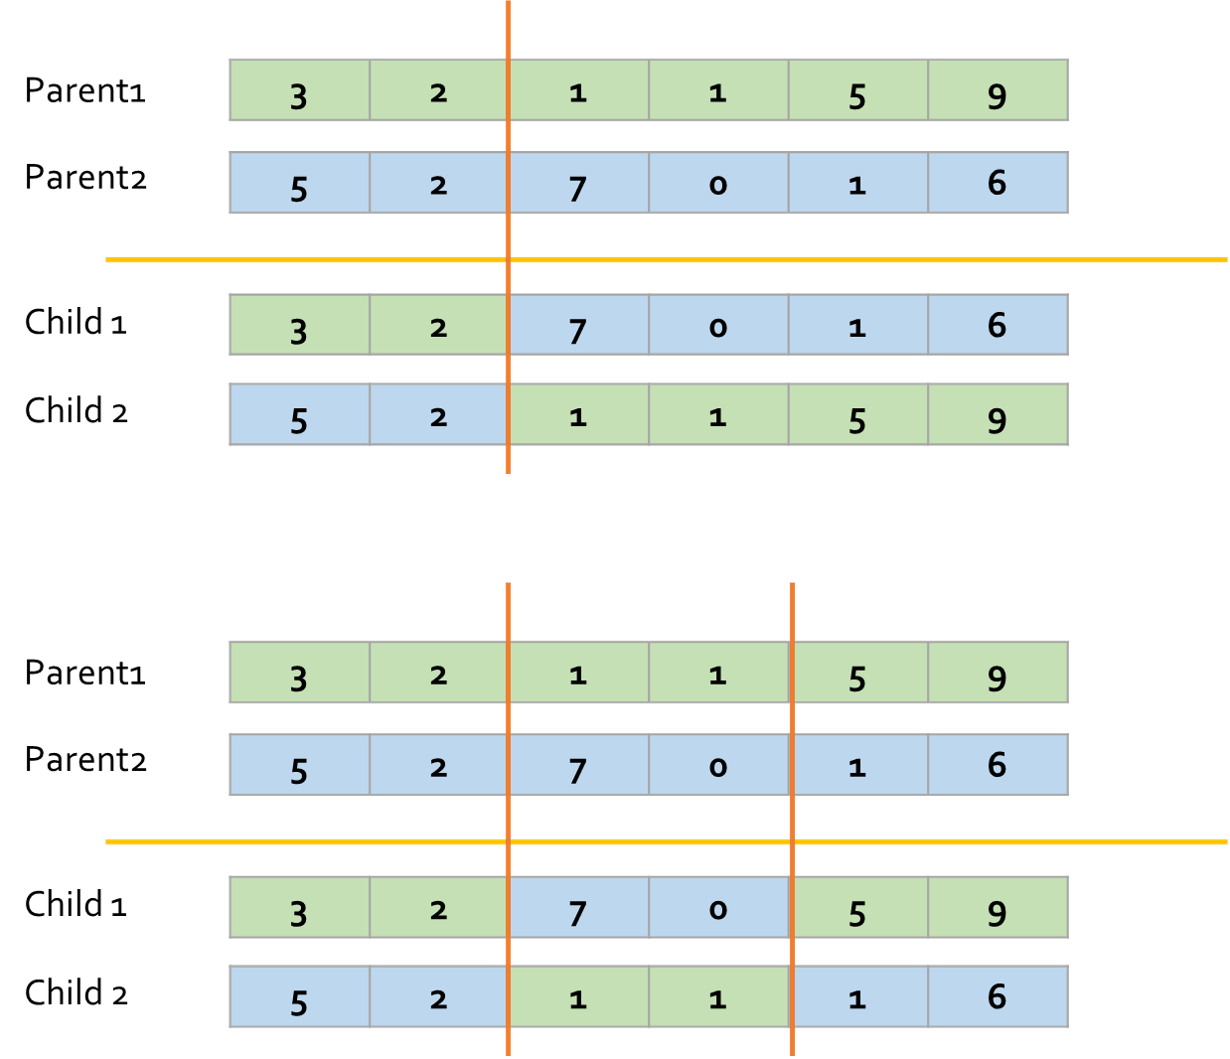
\includegraphics[width=0.8\textwidth]{img/crossover.png}
  \caption{Cruce de un punto (arriba) y cruce a dos puntos (abajo) aplicada a la mascara de individuos}
  \label{figure:crossover}
\end{figure}

\subsection{Operador de mutacion}
\label{subsection:mutation_operator}

La mutacion de los individuos de la poblacion ocurre solo al momento de hacer el
cruce de los mismos, es decir solo a los elementos nuevos se les aplica el
operador de mutacion, este operador puede modificar los siguientes elementos de
un individuo:
\begin{enumerate}
  \item La cantidad de piezas que conforman al individuo.
  \item El material del cual estan formados los elementos.
  \item El tipo de elemento que conforma a un individuo, es decir, modificar el
  valor del compuesto que forma parte del individuo.
  \item La posicion individual (\textit{x} o \textit{y}) de los compuestos.
\end{enumerate}

La manera en como se aplica el operador de mutacion se describe como sigue,
primeo al momento de generar al nuevo individuo se realiza un calculo de
porcentaje en donde se decide si tendra o no mutacion dependiendo del procentaje
de mutacion que se haya asignado al inicio del algoritmo, posteriormente en caso
de que el valor de porcentaje quede dentro del rango se toma para las
operaciones, esta mismas se explican de la manera siguiente.

Para mutar la cantida de compuestos en un individuo primero se realiza una
seleccion aleatoria entre las opciones de agregar o quitar compuestos,
posteriormente en caso de requerir agregar mas se realiza una seleccion
aleatoria de entre la cantidad de compuestos creados, estos mismos se integran
al final de la lista de compuestos del individuo. Para eliminar elementos de la
lista se realiza una corrida por todos los elementos y en cada uno se realiza
una probabilida de \textit{50\%} de sea borrado de la lista, un ejemplo de este
proceso se muestra en la figura \ref{figure:mutate_add_remove} en donde se
presenta una tabla que denota las posiciones de los compuestos en base a la
mascara, en este ejemplo se realizo una corrida para remover elementos (color
rojo) y una segunda para agregar nuevos compuestos (color verde).

\begin{figure}
  \centering
  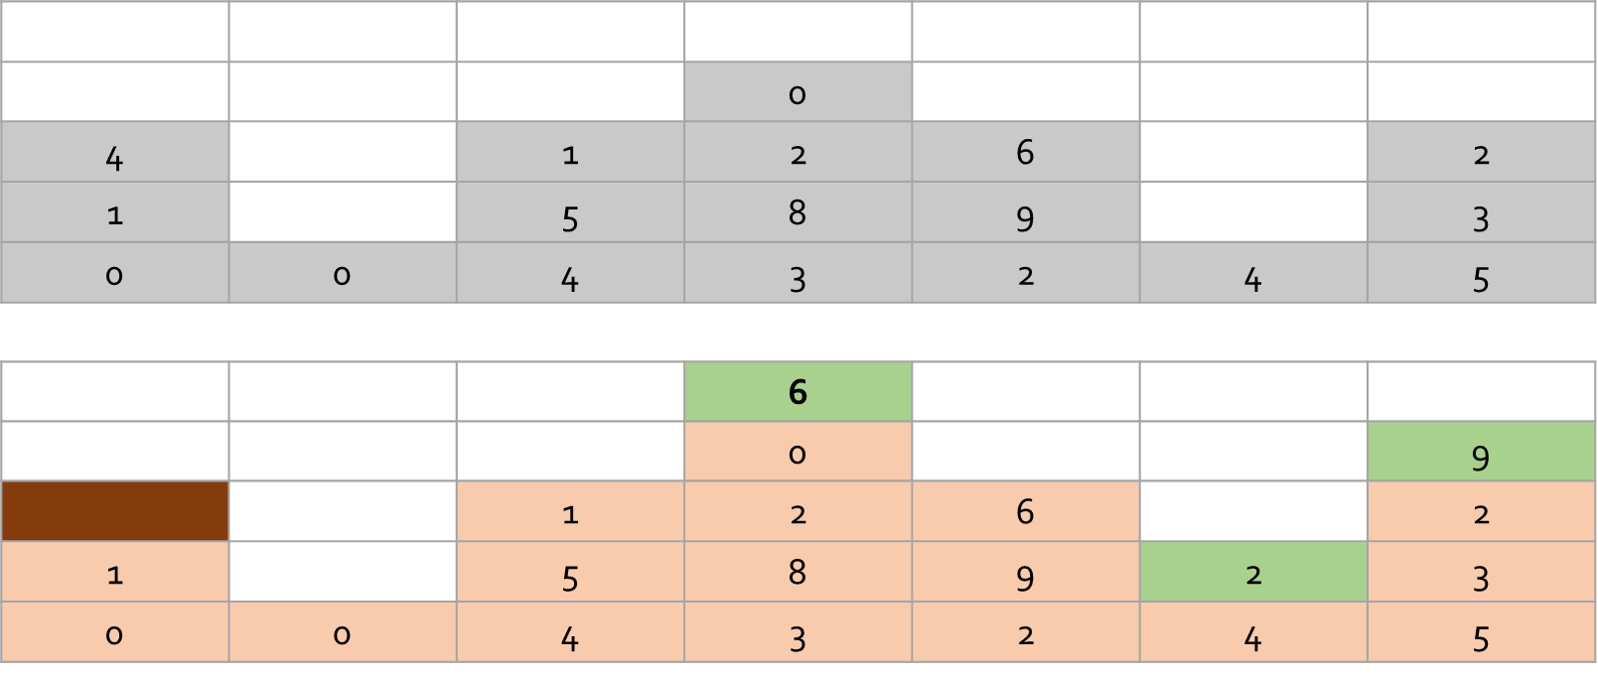
\includegraphics[width=0.8\textwidth]{img/mutation_add_remove.png}
  \caption{Ejemplo del operador de mutacion enfocado a remover y agregar compuestos}
  \label{figure:mutate_add_remove}
\end{figure}

La segunda mutacion se encarga de modificar el material del que estan
conformados los compuestos del individuo, la manera en como trabaja este proceso
es primero se selecciona aleatoriamente cuales compuestos seran modificados sin
repetir valores, posterioremente se modifica de manera aleatoria el valor que
define el tipo de material del que se conforma, para esto se toma en cuenta que
\textit{0} representa material de madera, \textit{1} representa material de
hielo y finalmente \textit{2} representa el material de piedra, debido a que el
juego solo acepta esta lista de compuestos no es posible asignar valores
diferentes a estos.

En la figura \ref{figure:mutate_composite} se muestra un ejemplo de la manera en
como opera la mutacion del tipo de compuesto, en este ejemplo 

\begin{figure}
  \centering
  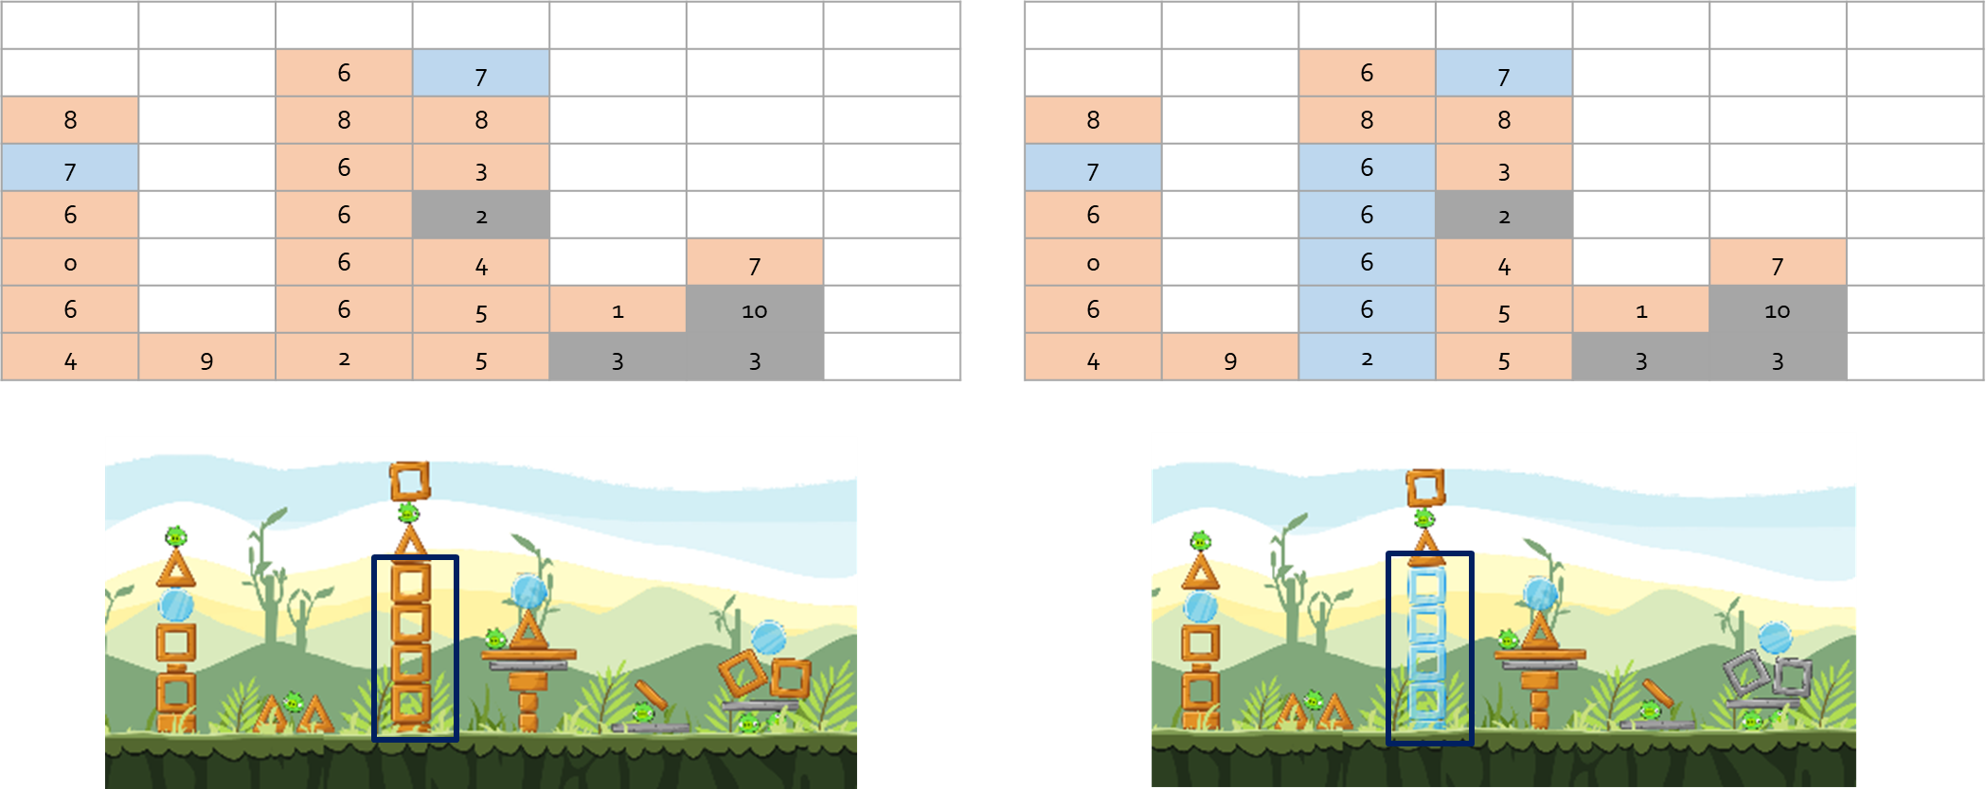
\includegraphics[width=0.9\textwidth]{img/mutation_material.png}
  \caption{Ejemplo del operador de mutacion enfocado a cambiar los compuestos asignados}
  \label{figure:mutate_composite}
\end{figure}